\section{Analysis of the classical convolution}
\label{sec:2.1}

In this section, we are exposing a few properties of the classical convolution that a generalization to graphs would likely try to preserve. For now let's consider a graph $G$ agnostically of its edges \ie $G \cong V$ is just the set of its vertices.

\subsection{Properties of the convolution}

Consider an edge-less grid graph \ie $G \cong \bbz^2$. By restriction to compactly supported signals, this case encompass the case of images.

\begin{definition}\textbf{Convolution on $\cs(\bbz^2)$}\\
Recall that the (discrete) convolution between two signals $s_1$ and $s_2$ over $\bbz^2$ is a binary operation in $\cs(\bbz^2)$ defined as:
\begin{align*}
\forall (a,b) \in \bbz^2, (s_1 \ast s_2) [a,b] & = \displaystyle \sum_i \sum_j s_1[i,j] \h{2} s_2[a-i, b-j]
\end{align*}
\label{def:conv}
\end{definition}

\begin{definition}\textbf{Convolution operator}\\
A \emph{convolution operator} is a function of the form $f_w: x \mapsto x \ast w$, where $x$ and $w$ are signals of domains for which the convolution $\ast$ is defined. When $\ast$ is not commutative, we differentiate the \emph{right} operator $x \mapsto x \ast w$ from the \emph{left} one $x \mapsto w \ast x$.
\end{definition}

The following properties of the convolution on $\bbz^2$ are of particular interest for our study.

\paragraph{Linearity}
Operators produced by the convolution are linear. So they can be used as linear parts of layers of neural networks.

\paragraph{Locality and weight sharing}
When $w$ is compactly supported on $K$, an impulse response $f_w(x)[a,b]$ amounts to a weighted aggregation of entries of $x$ in a neighborhood of $(a,b)$, called the \emph{Local Receptive Field} (LRF). The weight kernel $w$ used for the aggregation is fixed \wrt $(a,b)$, so that we say that the weights are shared.

\paragraph{Commutativity}
This convolution is commutative. However, it won't necessarily be the case on other domains.

\paragraph{Equivariance to translations}
Convolution operators are equivariant to translations. Below, we show that the converse of this result also holds with \thref{prop:equi}.

\subsection{Characterization on grid graphs}

We first define what a transformation of a domain is, and how it can be extended to signals defined on this domain.

\begin{definition}\textbf{Transformation}\\
A \emph{transformation} $f: V \rightarrow V$ is a function with same domain and codomain. The set of transformations is denoted $\Phi(V)$. The set of invertible transformations is denoted $\Phi^*(V) \subset \Phi(V)$. If $V$ is a linear space, the set of its linear transformation is denoted $\cl(V)$.
\end{definition}

\begin{remark}
Note that $\Phi^*(V)$ forms what is usually called the symmetric group of $V$.
\end{remark}

$\Phi^*(V)$ can \emph{move} signals of $\cs(V)$ by linear extension of its group action, as we explain with the lemma that follows.

\begin{lemma}\textbf{Extension of $\Phi^*(V)$ to $\cl(\cs(V))$}\\
An invertible transformation $f \in \Phi^*(V)$ can be extended linearly to the signal space $\cs(V)$, and we have:
\begin{gather*}
\forall s \in \cs(V), \forall v \in V, f(s)[v] = s[f^{-1}(v)]
\end{gather*}
\label{lem:extlin}
\end{lemma}
\begin{proof}
Let $s \in \cs(V), f \in \Phi^*(V), L_f \in \cl(\cs(V))$ \st $\forall v \in V, L_f(\delta_v) = \delta_{f(v)}$. Then, by linear decomposition of $s$ on the family of Dirac signals, we have:
\begin{align*}
L_f(s) & = \displaystyle\sum_{v \in V} s[v] \h{2} L_f(\delta_v)\\
       & = \displaystyle\sum_{v \in V} s[v] \h{2} \delta_{f(v)}\\
\text{So, }
\forall v \in V, L_f(s)[v] & = s[f^{-1}(v)]
\end{align*}
$L_f$ extends $f$ to $\cs(V)$. When there is no ambiguity, we use the same symbol for $f(.)$ and $L_f(.)$.
\end{proof}

For translations, we use the following formalism.

\begin{definition}\textbf{Translation on $\cs(\bbz^2)$}\\
A translation on $\bbz^2$ is defined as a transformation $t \in \Phi^*(\bbz^2)$ such that
\begin{gather*}
\exists (a,b) \in \bbz^2, \forall (x,y) \in \bbz^2, t(x,y) = (x+a,y+b)
\end{gather*}
By \lemref{lem:extlin}, it also acts on $\cs(\bbz^2)$ with the notation $t_{a,b}$ \ie
\begin{gather*}
\forall s \in \cs(\bbz^2), \forall (x,y) \in \bbz^2, t_{a,b}(s)[x,y] = s[x-a, y-b]
\end{gather*}
%For any set $E$, we denote by $\ct(E)$ its translations if they are defined.
\end{definition}

The next theorem fully characterizes convolution operators with their translational equivariance property. This can be seen as a discretization of a classic result from the theory of distributions~\citep{schwartz1957theorie}.

\begin{theorem}\textbf{Characterization of convolution operators on $\cs(\bbz^2)$}\\
On real-valued signals over $\bbz^2$, the class of linear transformations that are equivariant to translations is exactly the class of convolutive operations \ie
\begin{gather*}
\exists w \in \cs(\bbz^2), f = . \ast w \Leftrightarrow
\begin{cases}
 f \in \cl(\cs(\bbz^2))\\
 \forall t \in \ct(\cs(\bbz^2)), f \circ t = t \circ f
\end{cases}
\end{gather*}
\label{prop:equi}
\end{theorem}

\begin{proof}
The result from left to right is a direct consequence of the definitions:
\begin{align}
\forall s \in \cs(\bbz^2), \forall s' \in \cs(\bbz^2), & \forall (\alpha, \beta) \in \bbr^2,\forall (a,b) \in \bbz^2,\nonumber\\
 %f_w(s)[a,b] & = \displaystyle \sum_i \sum_j s[i,j] \h{2} w[a-i, b-j] \tag{definition}\\
 f_w(\alpha s + \beta s')[a,b] & = \displaystyle \sum_i \sum_j (\alpha s + \beta s')[i,j] \h{2} w[a-i, b-j]\nonumber\\
 & = \alpha f_w(s)[a,b] + \beta f_w(s')[a,b] \tag{linearity}\\
\forall s \in \cs(\bbz^2), \forall (x, y) \in \bbz^2, & \forall (a,b) \in \bbz^2,\nonumber\\
f_w \circ t_{x,y} (s)[a,b] & = \displaystyle \sum_i \sum_j t_{x,y}(s)[i,j] \h{2} w[a-i, b-j]\nonumber\\
 & = \displaystyle \sum_i \sum_j s[i - x,j - y] \h{2} w[a-i, b-j]\nonumber\\
 & = \displaystyle \sum_{i'} \sum_{j'} s[i',j'] \h{2} w[a - i' - x, b - j'- y]\label{eq:bij}\\
 & = f_w (s)[a - x,b - y]\nonumber\\
 & = t_{x,y} \circ f_w (s)[a,b] \tag{equivariance}
\end{align}
Now let's prove the result from right to left.

Let $f \in \cl(\cs(\bbz^2))$, $s \in \cs(\bbz^2)$ and we suppose that $f$ commutes with translations. By linear decomposition of $s$ on the family of Dirac signals, we have:
\begin{align*}
f(s) & = \displaystyle \sum_i \sum_j s[i,j] \h{2} f(\delta_{i,j})\\
 & = \displaystyle \sum_i \sum_j s[i,j] \h{2} f \circ t_{i,j} (\delta_{0,0})\\
 & = \displaystyle \sum_i \sum_j s[i,j] \h{2} t_{i,j} \circ f (\delta_{0,0})
\end{align*}
By denoting $w = f (\delta_{0,0}) \in \cs(\bbz^2)$, we obtain:
\begin{align}
\forall (a,b) \in \bbz^2, f(s)[a,b] & = \displaystyle \sum_i \sum_j s[i,j] \h{2} t_{i,j}(w)[a,b] \label{eq:conv}\\
 & = \displaystyle \sum_i \sum_j s[i,j] \h{2} w[a-i, b-j] \nonumber\\
\text{\ie } f(s) & = s \ast w \nonumber
\end{align}
\end{proof}

For example, on \figref{fig:cat}, $f$ is a convolution operator if, and only if, this diagram commutes.

\begin{figure}[h!t]
\begin{tikzpicture}
\node(a) at (0, 3) {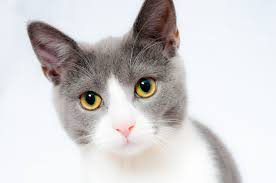
\includegraphics[width=0.22\linewidth,height=\textheight,keepaspectratio]{chapter2/cat.jpeg}};
\node(b) at (6, 3) {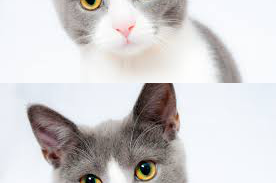
\includegraphics[width=0.22\linewidth,height=\textheight,keepaspectratio]{chapter2/cat_translated.jpeg}};
\node(c) at (0, 0) {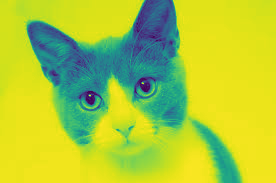
\includegraphics[width=0.22\linewidth,height=\textheight,keepaspectratio]{chapter2/cat_filtered.jpeg}};
\node(d) at (6, 0) {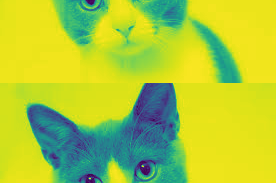
\includegraphics[width=0.22\linewidth,height=\textheight,keepaspectratio]{chapter2/cat_translated_filtered.jpeg}};
\path[->, thick] (a) edge node[above] {\textit{translation}} (b);
\path[->, thick] (a) edge node[left] {\scalebox{1.32}{$f$}} (c);
\path[->, thick] (b) edge node[right] {\scalebox{1.32}{$f$}} (d);
\path[->, thick] (c) edge node[above] {\textit{translation}} (d);
\end{tikzpicture}
\caption{Commutative diagram when $f$ is a convolution operator}
\label{fig:cat}
\end{figure}

\subsection{Usefulness of convolutions in deep learning}
\label{sec:cnnvsmlp}

\paragraph{Equivariance property of CNNs}
In deep learning, an important argument in favor of CNNs is that convolutional layers are equivariant to translations. Intuitively, that means that a detail of an object in an image should produce the same features independently of its position in the image.

\paragraph{Lossless superiority of CNNs over MLPs}
The converse result, as a consequence of~\thref{prop:equi}, is never mentioned in deep learning literature. However it is also a strong one. For example, let's consider a linear function that is equivariant to translations. Thanks to the converse result, we know that this function is a convolution operator parameterized by a weight vector $w$, $f_w : . \ast w$. If the domain is compactly supported, as in the case of images, we can break down the information of $w$ in a finite number $n_q$ of kernels $w_q$  with small compact supports of same size (for instance of size $2 \times 2$), such that we have $f_w = \sum_{q \in \seq{n_q}} f_{w_q}$. The convolution operators $f_{w_q}$ are all in the search space of $2 \times 2$ convolutional layers. In other words, every translational equivariant linear function can have its information parameterized by these layers. So that means that the reduction of parameters from an MLP to a CNN is done without loss of expressivity (provided the objective function is known to bear this property). Besides, it also helps the training to search in a much more confined space. For example, on CIFAR-$10$ (see description in \secref{sec:datasets}), CNNs reportedly attain up to 2.31\% error on classification \citep{yamada2018shakedrop}, while MLPs plateaued at 21.38\% \citep{lin2015}. Intuitively, the reason for this success is \emph{simplification by symmetry}: the supposed translational equivariance of the objective function is a symmetry that is exploited by the convolution layer to simplify its input.

\paragraph{Methodology for extending to general graphs}
Hence, in our construction, we will try to preserve the characterization from \thref{prop:equi} since it is mostly the reason why they are successful in deep learning. Note that other useful properties are also a consequence of this characterization. For example, the fact that convolutional layers have less parameters than a dense layer is also a consequence of this characterization.

%\subsection{Related works}

%\todo{}
% \todo{Maybe put this part in a section rather than a subsection. Finally rather put in in section 3.}





